% begin module area-between-curves-ex2
\begin{frame}
\begin{example} %[Example 2, p. 433]
\begin{columns}
\column{.35\textwidth}
\psset{xunit=1.5cm, yunit=1.5cm}
\begin{pspicture}(-0.5, -0.5)(1.5,2.7) 
\psframe*[linecolor=white](-0.5,-0.5)(1.7,2.7) 
\tiny 
\psaxes[ticks=none, labels=none]{<->}(0,0)(-0.5,-0.5)(1.5,2.5)
\psLabels{1.5}{2.5}
\psXTickWithLabel{1}{$1$}
\psYTickWithLabel{1}{$1$}
\psYTickWithLabel{2}{$2$}

\uncover<6->{
\psFullDot{1}{1}
\rput[bl](1.1,1){$(1,1)$}
\psFullDot{0}{0}
\rput[tl](0.05,-0.05){$(0,0)$}
}

\uncover<11->{ %
\pscustom*[linecolor=\psColorAreaUnderGraph]{ %
%Function formula: 2 (x)- ((x)^{2}) 
\psplot[linecolor=\psColorGraph, plotpoints=1000]{0}{1}{x 2 exp -1 mul x 2 mul add }
%Function formula: (x)^{2} 
\psplot[linecolor=\psColorGraph, plotpoints=1000]{1}{0}{x 2 exp }
} %
} %
\uncover<9->{ %
%Function formula: 2 (x)- ((x)^{2}) 
\rput[l](-0.4,0.7){$y=2 x- x^{2}$} 
\psplot[linecolor=\psColorGraph, plotpoints=1000]{-0.2}{1.5}{x 2 exp -1 mul x 2 mul add }
} %
\uncover<8->{ %
%Function formula: (x)^{2} 
\rput[r](1.3,2){$y=x^{2}$} 
\psplot[linecolor=\psColorGraph, plotpoints=1000]{-0.2}{1.5}{x 2 exp }
} %
\end{pspicture} 
%\ \only<handout:0| -5>{%
%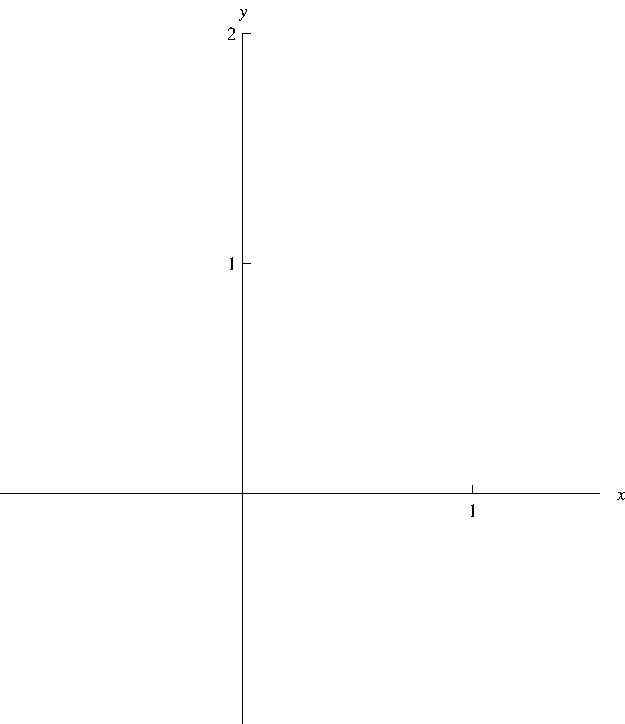
\includegraphics[height=4cm]{area-between-curves/pictures/06-01-ex2a.pdf}%
%}%  
%\only<handout:0| 6-7>{%
%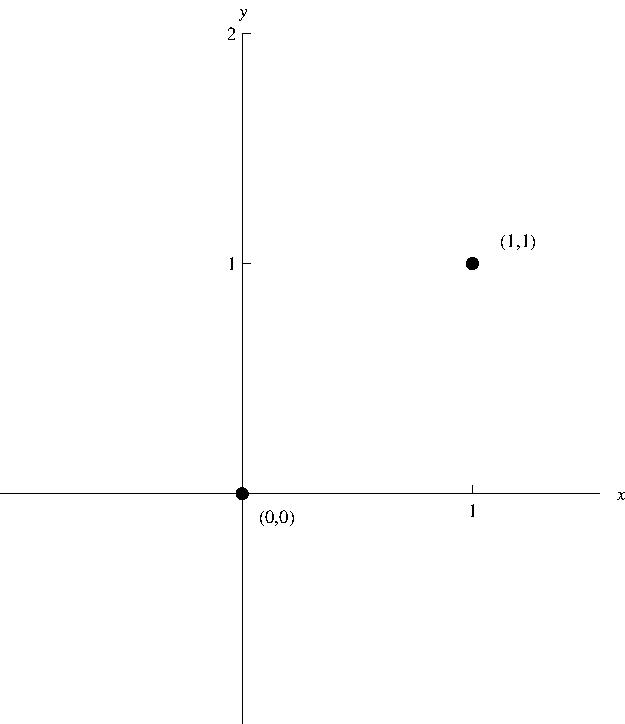
\includegraphics[height=4cm]{area-between-curves/pictures/06-01-ex2b.pdf}%
%}%  
%\only<handout:0| 8>{%
%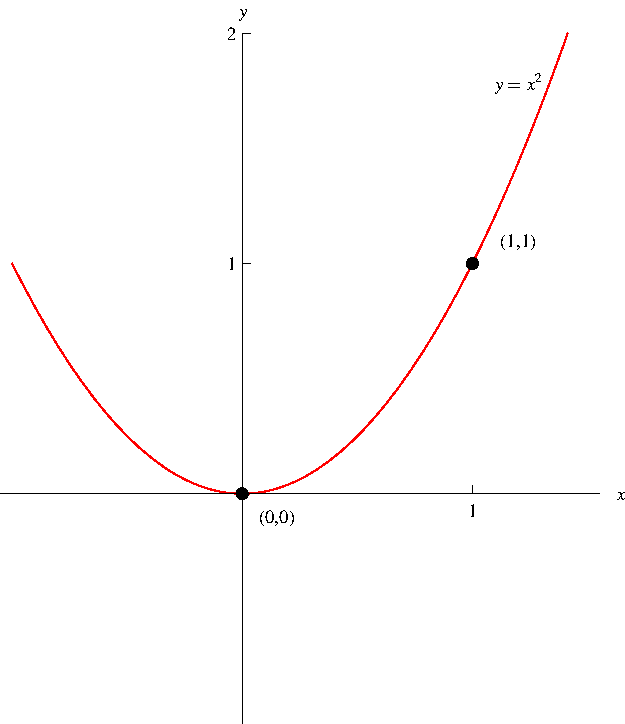
\includegraphics[height=4cm]{area-between-curves/pictures/06-01-ex2c.pdf}%
%}%  
%\only<handout:0| 9-10>{%
%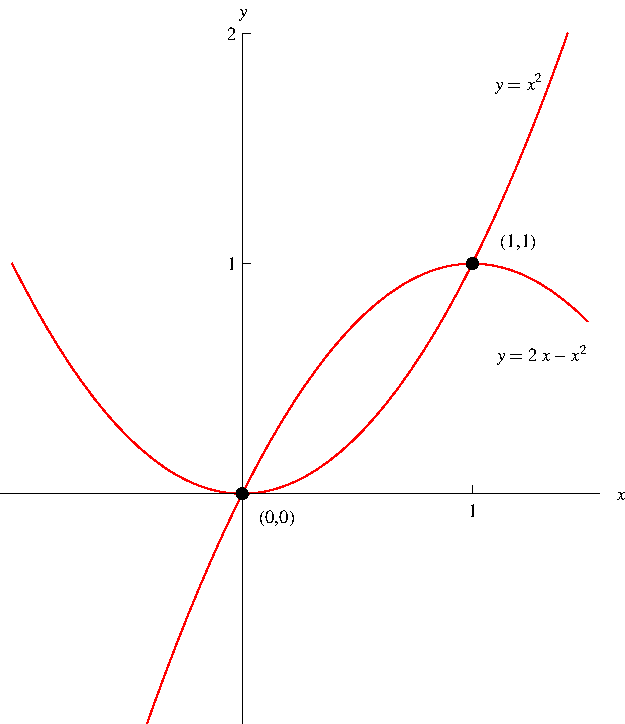
\includegraphics[height=4cm]{area-between-curves/pictures/06-01-ex2d.pdf}%
%}%  
%\only<11->{%
%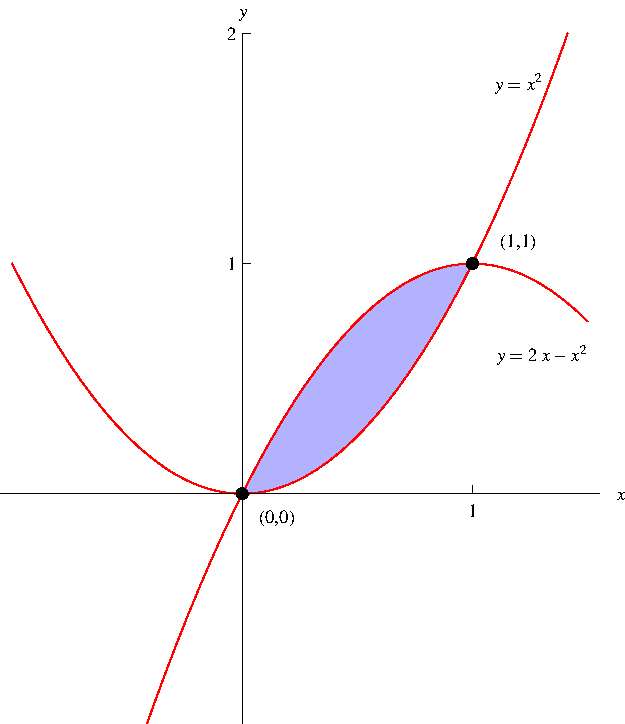
\includegraphics[height=4cm]{area-between-curves/pictures/06-01-ex2e.pdf}%
%}%  
\begin{enumerate}
\item<2->  Find the point of intersection.
\item<7->  Graph the functions.
\item<10->  Identify the region.
\item<12->  Integrate.
\end{enumerate}

\column{.65\textwidth}
Find the area of the region enclosed by the parabolas $\alert<handout:0| 8>{y =} \alert<handout:0| 3,8>{x^2}$ and $\alert<handout:0| 9>{y =} \alert<handout:0| 3,9>{2x - x^2}$.
\abovedisplayskip=0pt
\belowdisplayskip=0pt
\abovedisplayshortskip=0pt
\belowdisplayshortskip=0pt
\begin{align*}
\uncover<3->{\alert<handout:0| 3>{x^2}} & \uncover<3->{\alert<handout:0| 3>{=}}  \uncover<3->{\alert<handout:0| 3>{2x - x^2}} \\
\uncover<4->{0} & \uncover<4->{=}  \uncover<4->{2x - 2x^2} \uncover<5->{ = 2x(1 - x)} \\
\uncover<6->{x} & \uncover<6->{=}  \uncover<6->{0 \text{ or } 1.}
\end{align*}
\begin{align*}
\uncover<13->{A} & \uncover<13->{=}  \uncover<13->{\int_0^1 (2x - 2x^2) \diff x} \uncover<14->{ = 2\int_0^1 (x - x^2) \diff x} \\
 & \uncover<15->{=}  \uncover<15->{2\left[ \frac{x^2}{2} - \frac{x^3}{3}\right]_0^1} \uncover<16->{ = 2\left( \frac{1}{2} - \frac{1}{3}\right)} \uncover<17->{ = \frac{1}{3}.}
\end{align*}
\end{columns}
\end{example}
\end{frame}
% end module area-between-curves-ex2
